%%
%% Calculator GroupLab (c) 2021-22 Christopher A. Bohn
%%
%% Licensed under the Apache License, Version 2.0 (the "License");
%% you may not use this file except in compliance with the License.
%% You may obtain a copy of the License at
%%     http://www.apache.org/licenses/LICENSE-2.0
%% Unless required by applicable law or agreed to in writing, software
%% distributed under the License is distributed on an "AS IS" BASIS,
%% WITHOUT WARRANTIES OR CONDITIONS OF ANY KIND, either express or implied.
%% See the License for the specific language governing permissions and
%% limitations under the License.
%%

%%
%% (c) 2021 Christopher A. Bohn
%%

\documentclass[12pt]{article}

\usepackage{fullpage}
\usepackage{fancyhdr}
\usepackage[procnames]{listings}
\usepackage{hyperref}
\usepackage{textcomp}
\usepackage{bold-extra}
\usepackage[dvipsnames]{xcolor}
\usepackage{etoolbox}


% Customize the semester (or quarter) and the course number

\newcommand{\courseterm}{Spring 2022}
\newcommand{\coursenumber}{CSCE 231}

% Customize how a typical lab will be managed;
% you can always use \renewcommand for one-offs

\newcommand{\runtimeenvironment}{your account on the \textit{csce.unl.edu} Linux server}
\newcommand{\filesource}{Canvas or {\footnotesize$\sim$}cse231 on \textit{csce.unl.edu}}
\newcommand{\filesubmission}{Canvas}

% These are placeholder commands and will be renewed in each lab

\newcommand{\labnumber}{}
\newcommand{\labname}{Lab \labnumber\ Assignment}
\newcommand{\shortlabname}{}
\newcommand{\duedate}{}

% Individual or team effort

\newcommand{\individualeffort}{This is an individual-effort project. You may discuss concepts and syntax with other students, but you may discuss solutions only with the professor and the TAs. Sharing code with or copying code from another student or the internet is prohibited.}
\newcommand{\teameffort}{This is a team-effort project. You may discuss concepts and syntax with other students, but you may discuss solutions only with your assigned partner(s), the professor, and the TAs. Sharing code with or copying code from a student who is not on your team, or from the internet, is prohibited.}
\newcommand{\freecollaboration}{In addition to the professor and the TAs, you may freely seek help on this assignment from other students.}
\newcommand{\collaborationrules}{}

% Do you care about software engineering?

\providebool{allowspaghetticode}

\setbool{allowspaghetticode}{false}

\newcommand{\softwareengineeringfrontmatter}{
    \ifboolexpe{not bool{allowspaghetticode}}{
        \section*{No Spaghetti Code Allowed}
        In the interest of keeping your code readable, you may \textit{not} use
        any \lstinline{goto} statements, nor may you use any \lstinline{break}
        statements to exit from a loop, nor may you have any functions
        \lstinline{return} from within a loop.
    }{}
}

\newcommand{\spaghetticodepenalties}[1]{
    \ifboolexpe{not bool{allowspaghetticode}}{
        \penaltyitem{1}{for each \lstinline{goto} statement, \lstinline{break}
            statement used to exit from a loop, or \lstinline{return} statement
            that occurs within a loop.}
    }{}
}

% You shouldn't need to customize these,
% but you can if you like

\lstset{language=C, tabsize=4, upquote=true, basicstyle=\ttfamily}
\newcommand{\function}[1]{\textbf{\lstinline{#1}}}
\setlength{\headsep}{0.7cm}
\hypersetup{colorlinks=true}

\newcommand{\startdocument}{
    \pagestyle{fancy}
    \fancyhf{}
    \lhead{\coursenumber}
    \chead{\ Lab \labnumber: \labname}
    \rhead{\courseterm}
    \cfoot{\shortlabname-\thepage}

	\begin{document}
	\title{\ Lab \labnumber}
	\author{\labname}
	\date{Due: \duedate}
	\maketitle

    \textit{\collaborationrules}
}

\newcommand{\rubricitem}[2]{\item[\underline{\hspace{1cm}} +#1] #2}
\newcommand{\bonusitem}[2]{\item[\underline{\hspace{1cm}} Bonus +#1] #2}
\newcommand{\penaltyitem}[2]{\item[\underline{\hspace{1cm}} -#1] #2}

%%
%% labs/common/semester.tex
%% (c) 2021-22 Christopher A. Bohn
%%
%% Licensed under the Apache License, Version 2.0 (the "License");
%% you may not use this file except in compliance with the License.
%% You may obtain a copy of the License at
%%     http://www.apache.org/licenses/LICENSE-2.0
%% Unless required by applicable law or agreed to in writing, software
%% distributed under the License is distributed on an "AS IS" BASIS,
%% WITHOUT WARRANTIES OR CONDITIONS OF ANY KIND, either express or implied.
%% See the License for the specific language governing permissions and
%% limitations under the License.
%%


% Customize the semester (or quarter) and the course number

\newcommand{\courseterm}{Fall 2022}
\newcommand{\coursenumber}{CSCE 231}

% Customize how a typical lab will be managed;
% you can always use \renewcommand for one-offs

\newcommand{\runtimeenvironment}{your account on the \textit{csce.unl.edu} Linux server}
\newcommand{\filesource}{Canvas or {\footnotesize$\sim$}cse231 on \textit{csce.unl.edu}}
\newcommand{\filesubmission}{Canvas}

% Customize for the I/O lab hardware

\newcommand{\developmentboard}{Arduino Nano}
%\newcommand{\serialprotocol}{SPI}
\newcommand{\serialprotocol}{I2C}
%\newcommand{\displaymodule}{MAX7219digits}
%\newcommand{\displaymodule}{MAX7219matrix}
\newcommand{\displaymodule}{LCD1602}

\setbool{usedisplayfont}{true}

\newcommand{\obtaininghardware}{
    The EE Shop has prepared ``class kits'' for CSCE 231; your class kit costs \$30.
    The EE Shop is located at 122 Scott Engineering Center and is open M-F 7am-4pm. You do not need an appointment.
    You may pay at the window with cash, with a personal check, or with your NCard.
    The EE shop does \textit{not} accept credit cards.
}

% Update to reflect the CS2 course(s) at your institute

\newcommand{\cstwo}{CSCE~156, RAIK~184H, or SOFT~161}

% Do you care about software engineering?

\setbool{allowspaghetticode}{false}

% Which assignments are you using this semester, and when are they due?

\newcommand{\pokerlabnumber}{1}
\newcommand{\pokerlabcollaboration}{
    Sections~\ref{sec:connecting}, \ref{sec:terminology}, \ref{sec:gettingstarted}, \ref{subsec:typesofpokerhands}, and~\ref{subsec:studythecode}: \freecollaboration
    Sections~\ref{sec:completingcard} and~\ref{subsec:completepoker}: \individualeffort
}
\newcommand{\pokerlabdue}{Week of August 29, before the start of your lab section}

\newcommand{\keyboardlabnumber}{2}
\newcommand{\keyboardlabcollaboration}{\individualeffort}
\newcommand{\keyboardlabdue}{Week of January 31, before the start of your lab section}

\newcommand{\pointerlabnumber}{3}
\newcommand{\pointerlabcollaboration}{\individualeffort}
\newcommand{\pointerlabdue}{Week of February 7, before the start of your lab section}

\newcommand{\integerlabnumber}{4}
\newcommand{\integerlabcollaboration}{\individualeffort}
\newcommand{\integerlabdue}{Week of February 14, before the start of your lab section}

\newcommand{\floatlabnumber}{5}
\newcommand{\floatlabcollaboration}{\individualeffort}
\newcommand{\floatlabdue}{soon}

\newcommand{\addressinglabnumber}{6}
\newcommand{\addressinglabcollaboration}{\individualeffort}
\newcommand{\addressinglabdue}{Week of February 28, before the start of your lab section}

%bomblab was 7
%attacklab was 8

\newcommand{\pollinglabnumber}{9}
\newcommand{\pollinglabcollaboration}{\individualeffort}
\newcommand{\pollinglabdue}{Week of April 11, before the start of your lab section}
\newcommand{\pollinglabenvironment}{your \developmentboard-based class hardware kit}

\newcommand{\ioprelabnumber}{\pollinglabnumber-prelab}
\newcommand{\ioprelabcollaboration}{\freecollaboration}
\newcommand{\ioprelabdue}{Before the start of your lab section on April 5 or 6}

\newcommand{\interruptlabnumber}{10}
\newcommand{\interruptlabcollaboration}{\individualeffort}
\newcommand{\interruptlabdue}{Week of April 18, before the start of your lab section}
\newcommand{\interruptlabenvironment}{your \developmentboard-based class hardware kit}

\newcommand{\capstonelab}{ComboLock}    % this will come into play when we generalize capstonelab
\newcommand{\capstonelabnumber}{11}
\newcommand{\capstonelabcollaboration}{\teameffort}
\newcommand{\capstonelabdue}{Week of May 2, Before the start of your lab section\footnote{See Piazza for the due dates of teams with students from different lab sections.}}
\newcommand{\capstonelabenvironment}{your \developmentboard-based class hardware kit}

\newcommand{\memorylabnumber}{12}
\newcommand{\memorylabcollaboration}{This is an individual-effort project. You may discuss the nature of memory technologies and of memory hierarchies with classmates, but you must draw your own conclusions.}
\newcommand{\memorylabdue}{Week of May 2, at the end of your lab section}
\newcommand{\memorylabenvironment}{your \developmentboard-based class hardware kit and your account on the \textit{csce.unl.edu} Linux server}

% Labs not used this semester

\newcommand{\concurrencylabnumber}{XX}
\newcommand{\concurrencylabcollaboration}{\individualeffort}
\newcommand{\concurrencylabdue}{not this semester}

\newcommand{\ssbcwarmupnumber}{XX}
\newcommand{\ssbcwarmupcollaboration}{\freecollaboration}
\newcommand{\ssbcwarmupdue}{not this semester}

\newcommand{\ssbcpollingnumber}{XX}
\newcommand{\ssbcpollingcollaboration}{\individualeffort}
\newcommand{\ssbcpollingdue}{not this semester}

\newcommand{\ssbcinterruptnumber}{XX}
\newcommand{\ssbcinterruptcollaboration}{\individualeffort}
\newcommand{\ssbcinterruptdue}{not this semester}

\usepackage{graphicx}
%\usepackage{media9}
\usepackage{addfont}
\addfont{OT1}{d7seg}{\dviiseg}
% \addfont{OT1}{deseg}{\deseg}
%\usepackage[normalem]{ulem}
%\usepackage{subfig}
\usepackage{wrapfig}
%\usepackage{animate}
% \usepackage{multicol}
\usepackage{enumitem}

\renewcommand{\labnumber}{\capstonelabnumber}
\renewcommand{\labname}{Implementing a 4-Function Calculator using Interrupts}
\renewcommand{\shortlabname}{interrupt-driven i/o -- calculator -- grouplab}
\renewcommand{\collaborationrules}{\capstonelabcollaboration}
\renewcommand{\duedate}{\capstonelabdue}
\newcommand{\nano}{\developmentboard} % TODO: replace \nano with \developmentboard
\renewcommand{\runtimeenvironment}{\capstonelabenvironment}
\pagelayout
\begin{document}
\labidentifier

In this assignment, you will write code for \runtimeenvironment\ that will use
interrupts from external devices and from a timer to drive some of the logic
for a four-function calculator.

\begin{figure}[h]
    \centering
    
\includegraphics[width=10cm]{MomMomMom}
    \caption{Interrupts. \tiny Image by 20th Century Fox Television}
\end{figure}

The instructions are written assuming you will edit the code in the Arduino IDE
and run it on \runtimeenvironment, constructed according to the pre-lab
instructions. If you wish, you may edit the code in a different environment;
however, our ability to provide support for problems with other IDEs is limited.

\section*{Learning Objectives}

After successful completion of this assignment, students will be able to:
\begin{itemize}
\item Work collaboratively on a hardware/software project
\item Use tables from a datasheet to determine the bit vectors needed to
    configure I/O devices
\item Configure a hardware timer to generate interrupts
\item Register an interrupt service routine for an interrupt vector
\item Register an interrupt service routine using a higher abstraction
\item Use interrupt-driven I/O to design and implement a simple embedded system
\end{itemize}

\subsection*{Continuing Forward}

This penultimate lab assignment does not contribute to the final lab assignment.
By integrating elements of what you learned in this course to design a small
embedded system, you will show how much progress you have made this semester.

\section*{During Lab Time}

During your lab period, the TAs will demonstrate how to use tables from a datasheet to construct bit vectors.
Coordinate with your group partner(s) to decide on your working arrangements.
Unless you're only going to work on the assignment when you're together, you may want to set up a \textit{private} Git repository that is shared with your partner(s).
With your partner(s), think through your system's design and begin implementing it.
The TAs will be available for questions.

\softwareengineeringfrontmatter

\section{Scenario}

``I have various teams working on different projects around here to improve security,'' Archie reminds you.
He glances toward the Zoo's labs, where there's now a guy who looks like the actor who portrayed the fictional actor who portrayed the Norse god Odin, trying to avoid children while wistfully talking about raising rabbits in Montana.
You briefly wonder why there are children someplace where there are also carnivorous megafauna, and then you remember that you work at a petting zoo.
``What I need your team to do,'' Archie continues, ``is make a four-function calculator so that we can quickly and easily determine whether we have the correct number of specimens, or if any are missing.''

\section{Lab Overview}

Please familiarize yourself with the entire assignment before beginning.
Section~\ref{sec:FunctionalSpecification} has the functional specification of the system you will develop.
Obviously, detecting inputs is necessary before being able to implement any other requirements, and section~\ref{sec:DetectingInputs} describes detecting inputs using interrupts.
While you're in an interrupt frame of mind, you might go ahead and implement the display-timeout requirement; section~\ref{sec:TimerInterrupts} describes configuring a timer to do so.
Alternately, you could implement the rest of the calculator's features before tackling the display-timeout requirement.

Note that Figure~\ref{fig:StateDiagram} depicts the ``normal'' behavior for the system as a state diagram.
You might find that designing your software as a state machine may make it easier to implement your system.


\subsection{Interrupt-Driven Input/Output -- A Different but Familiar Programming Paradigm}

In PollingLab you used polling to determine when to respond to a pushbutton or a key on the keypad being pressed.
In this lab, you will rely on interrupts to let your code know when it needs to respond to a pushbutton or a key on the keypad being pressed, and you will rely on interrupts to let your code know when a certain amount of time has passed.

\vspace{.25cm}

Most of the code you wrote in the earlier lab assignments for this courses used
imperative programming: you, the programmer, had full control over changes to
the program state. In PollingLab, you stretched this model to something
resembling shared-memory concurrent programming: you still had full control
over changes to the program state of your program's flow of control, but your
program periodically read variables (memory-mapped input registers) that could be
changed by another flow of control (the physical world).

In this lab assignment, you will write code that reacts to things happening in
the physical world; your code program state will not change except in reaction to interrupts.
Conceptually, this isn't very different from event-driven programming that you
learned in \cstwo. While configuring the hardware timer is a little more complex
than configuring a GUI framework's timer, handling a timer interrupt is very
much like writing an \function{onTimeout()} event handler. Similarly, handling
a change in a pushbutton's position is very much like writing an
\function{onMouseClick} event handler. Your code is not focused on \textit{when}
the button is pressed or released, nor even on \textit{detecting} that a button
has been pressed or released; it is focused solely on \textit{what should happen}
when the button is pressed or released.

\subsection{Constraints}

% \section{Constraints}\label{sec:Constraints}

You may re-use your code that uses memory-mapped I/O registers, or you can use
functions provided by the CowPi library to read from and write to pins.

You may \textit{not} poll the matrix keypad nor the pushbuttons to determine
if they have been pressed. You must use interrupts to determine if a key or
button has been pressed. Once a press has been detected, you may scan the
matrix keypad or read the pushbuttons to determine which key or button has
been pressed.

You may poll the left switch to determine if its position has changed;
however, the specification has been written such that your code should only
need to occasionally check the switch's position rather than polling it for
changes.

% While it is possible to configure the SPI hardware to generate an interrupt
% after the content of the SPI Data Register is transmitted, you may use your
% \function{send_data()} function that polls the \texttt{SPIF} bit.

While it is possible to configure the I$^2$C hardware to generate an interrupt
after the content of the TWI Data Register is transmitted, you may use your
\function{send_halfbyte()} function that polls the \texttt{TWINT} bit, or you may
use the Cow Pi library's default implementation.

\subsubsection{Constraints on the Arduino core}

You may use \function{attachInterrupt()} and \function{digitalPinToInterrupt()} to register interrupt handlers.
You may use the \function{delayMicroseconds()} function to introduce a 1--2$\mu$s delays if necessary.
You may (but are not required to) use \function{Serial.print()} and \function{Serial.println()} instead of \function{printf()} if you wish.

While you may use \function{millis()} for debouncing, you may \textit{not} use
\function{millis()} nor \function{micros()} to implement the display timeout.
You must use an interrupt from the ATmega328's Timer1 or Timer2 as part of
implementing the display timeout.

You may not use any other libraries, functions, macros, types, or constants from the Arduino core.\footnote{\url{https://www.arduino.cc/reference/en/}}

\subsubsection{Constraints on AVR-libc}

You may use any AVR-specific functions, macros, types, or constants of avr-libc.\footnote{\url{https://www.nongnu.org/avr-libc/user-manual/index.html}}

\subsubsection{Constraints on the CowPi library}

You may use any functions that are described in Section~2 of the Cow Pi
datasheet, and you may use any data structures provided by the CowPi library.

\subsubsection{Constraints on other libraries}

You may not use any libraries beyond those explicitly identified here.

\subsubsection{Constraints on code from earlier assignments}

You may use any code written by you or your partner(s), including code that you or your partner(s) wrote for this course.


\section{Four-Function Calculator Specification} \label{sec:FunctionalSpecification}

\subsection*{Integer Calculator}

\begin{enumerate}
\item \label{spec:IntegerCalculator} The calculator shall be an
    infix\footnote{\url{https://en.wikipedia.org/wiki/Calculator_input_methods\#Infix_notation}}
    decimal calculator capable of performing addition, subtraction,
    multiplication, and division.
    \begin{itemize}
    % \item If only integer behavior is implemented, then division shall be
    %     integer division; \textit{i.e.}, the fractional portion of quotients
    %     values shall be truncated.
    \item Division shall be integer division; \textit{i.e.}, the fractional portion of quotients values shall be truncated.
    \end{itemize}
\item \label{spec:NoDecimalPoint} A decimal point shall not be displayed. Digit-separating commas are optional, neither required nor prohibited.
\item Each arithmetic operation shall use two operands, referred in this
    specification as \textit{operand1} and \textit{operand2}.
    \begin{itemize}
    \item Because no further history of operands is maintained, the algebraic
        order of operations is not preserved.
    \item The value of \textit{operand1} can only be changed as the result of a
        calculation or by clearing its value.
    \item The value of \textit{operand2} is ``built'' through keypresses on the
        matrix keypad.
    \item \textit{operand1} and \textit{operand2} are defined in the problem
        domain. Your solution space might not have direct corollaries (for
        example, in the problem domain, \textit{operand2} can be undefined,
        which is not a characteristic of any number types in C).
    \end{itemize}

% \item The \textbf{7-segment display module} shall display \textit{operand1}'s
%     value except when building \textit{operand2}, except when an error
%     condition is present, and except when the display is disabled.

\item The \textbf{display module} shall display the decimal representation of \textit{operand1}'s value on the top row, right-justified, except when an error condition is present.
\item If \textit{operand2} has a defined value (is being built) then the \textbf{display module} shall display the decimal representation of \textit{operand2}'s value on the bottom row, right-justified, except when an error condition is present. If \textit{operand2} does not have a defined value then the visual space for \textit{operand2}'s value shall be blank.
\item \label{spec:displayOperation} If an operation is specified, then the character for that operation ($+, -, \times, \div$) shall be displayed in the lower-left corner of the \textbf{display module}. If no operation is specified, then the visual space for the operation's character shall be blank.

\item Initially, \textit{operand1} shall hold the value 0, \textit{operand2}
    shall have no defined value, and no arithmetic operation shall be specified.
\item \label{spec:BuildingValue} When building \textit{operand2}:
    \begin{enumerate}
    % \item When the user starts to build \textit{operand2}, \textit{operand1}
    %     shall no longer be displayed. Instead, the value being built shall be
    %     displayed.
    \item Except as otherwise specified in requirement~\ref{spec:Wakening},
        whenever the user presses a numeral button on the \textbf{matrix
        keypad}, the corresponding digit shall be displayed in the
        least-significant position of the value on the \textbf{display module},
        and any digits already displayed shall increase in significance by one
        order of magnitude. For example, if \display{234} is displayed and the
        user presses \texttt{5} then \display{2345} shall be displayed.
    \item Except as otherwise specified in requirement~\ref{spec:Wakening},
        whenever the user presses the \textbf{left pushbutton}, the value being
        built shall be negated, and the visual representation of the number shall reflect this.
        \begin{itemize}
        \item If \textit{operand2} has a defined value (is being built) then
            \textit{operand2} shall be negated.
        \item If \textit{operand2} has no defined value (\textit{operand2} is not displayed, but \textit{operand1} is) then \textit{operand1} shall be negated.
        \end{itemize}

    % \item In no case shall the calculator allow the user to input a value
    %     requiring more digits than can be displayed on the \textbf{7-segment
    %     display module}. If the user attempts to enter a value that requires
    %     more digits, then the value shall remain unchanged.

    \item In no case shall the calculator allow the user to input a value requiring more than nine (9) digits, (the negative sign, if present, is not considered to be one of these digits). If the user attempts to enter a value that requires more digits, then the value shall remain unchanged.

    \end{enumerate}
\item \label{spec:Negative} If a negative value is displayed, the negative sign
    shall be displayed immediately to the left of the most-significant digit
    being displayed. For example, \display{-456} is correctly displayed, but
    \display{-\phantom{xxxx}456} is not correctly displayed.
\item \label{spec:Positive} A positive sign shall not be displayed as part of a
    positive value.
\item \label{spec:LeadingZeroes} Leading 0s shall not be displayed. For
    example, \display{782} is correctly displayed, but \display{00000782} is
    not correctly displayed. However, when the value to be displayed is 0, then
    \display{0} shall be displayed.
\item The \texttt{A} button indicates addition. The \texttt{B} button indicates
    subtraction. The \texttt{C} button indicates multiplication. The \texttt{D}
    button indicates division. The \texttt{\#} button directs that the
    calculation shall be executed without specifying another arithmetic
    operation.
\item Except as otherwise specified in requirement~\ref{spec:Wakening}, when
    the user presses the \texttt{\#} button, directing that the calculation is
    to be executed, the previously-specified operation shall be
    performed, the resulting value shall become \textit{operand1} (and shall be
    displayed on the top row), and there shall no longer be a valid \textit{operand2} (and thus cannot be displayed) nor a specified operation (and thus cannot be displayed). If
    there was no previously-specified operation, then \textit{operand2} shall
    become \textit{operand1}, and there shall no longer be a valid
    \textit{operand2}.
\item Except as otherwise specified in requirement~\ref{spec:Wakening}, when
    the user presses an operation button (\texttt{A}-\texttt{D}), the
    \underline{previously}-specified operation shall be performed, the
    resulting value shall become \textit{operand1} (and shall be displayed on the top row),
    there shall no longer be a valid \textit{operand2} (and thus cannot be displayed), and the \underline{next} operation
    to be performed shall be that which corresponds to the button pressed. If
    there was no previously-specified operation, then \textit{operand2} shall
    become \textit{operand1}, \textit{operand2} shall no longer have a defined
    value, and the \underline{next} operation to be performed shall be that
    which corresponds to the button pressed. In accordance with requirement~\ref{spec:displayOperation}, the \underline{next} operation shall be displayed.
    \begin{itemize}
    \item If the resulting value (\textit{operand1}) is too great to be
        displayed, the \textbf{display module} shall display
        \display{Error}.
    \item If \textit{operand2} is 0 and the operation is division, the
        \textbf{display module} shall display \display{Error}.
    \end{itemize}
\item The calculator shall not support scientific notation, neither for operand
    entry nor for displaying a result.
\item Except as otherwise specified in requirement~\ref{spec:Wakening},
    whenever the user presses the \textbf{right pushbutton}:
    \begin{enumerate}
    \item If \textit{operand2} is being built, then \textit{operand2} shall be
        reset to no defined value, the next operation (if any) shall be
        cleared, and \textit{operand1} shall be displayed.
    \item If \textit{operand2} is not being built, then \textit{operand1} shall
        be reset to 0 (and 0 shall be displayed), and the next operation (if
        any) shall be cleared.
    \end{enumerate}

% \item Display timeout: If no button or key has been pressed for a designated
%     amount of time, the \textbf{7-segment display module} shall go blank;
%     however, \textit{operand1}, \textit{operand2} being built (if any), and the
%     next operation (if any) shall be retained. When the \textbf{left switch} is
%     in the left position, the designated time is \underline{exactly 20
%     seconds}; when the \textbf{left switch} is in the right position, the
%     designated time is \underline{exactly 7.5 seconds}.
\item Display timeout: If no button or key has been pressed for a designated
    amount of time, the \textbf{display module}'s backlight shall deluminate;
    however, \textit{operand1}, \textit{operand2} being built (if any), and the
    next operation (if any) shall be retained. When the \textbf{left switch} is
    in the left position, the designated time is \underline{exactly 20
    seconds}; when the \textbf{left switch} is in the right position, the
    designated time is \underline{exactly 7.5 seconds}.
    \begin{itemize}
    \item Do not place the microcontroller in Idle mode, nor any other Sleep
        mode.
    \end{itemize}

% \item \label{spec:Wakening} If the display has timed out, then pressing any key
%     or button will cause the display to resume displaying its previous output.
%     The key/button press that takes the display out of its timed-out mode shall
%     not otherwise affect the system's state; specifically, it shall not
%     contribute to \textit{operand2}'s value, it shall not cause an operation to
%     be executed, it shall not specify an operation to be performed, nor shall
%     it clear any operands or specified operations.
\item \label{spec:Wakening} If the display has timed out, then pressing any key
    or button will cause the backlight to illuminate.
    The key/button press that takes the display out of its timed-out mode shall
    not otherwise affect the system's state; specifically, it shall not
    contribute to \textit{operand2}'s value, it shall not cause an operation to
    be executed, it shall not specify an operation to be performed, nor shall
    it clear any operands or specified operations.
\end{enumerate}

Figure~\ref{fig:StateDiagram} depicts a problem-space state diagram of the
4-function integer calculator, not including too-great values, and not
including the display's time-out and resume-display behavior.

\begin{figure}
    \centering
    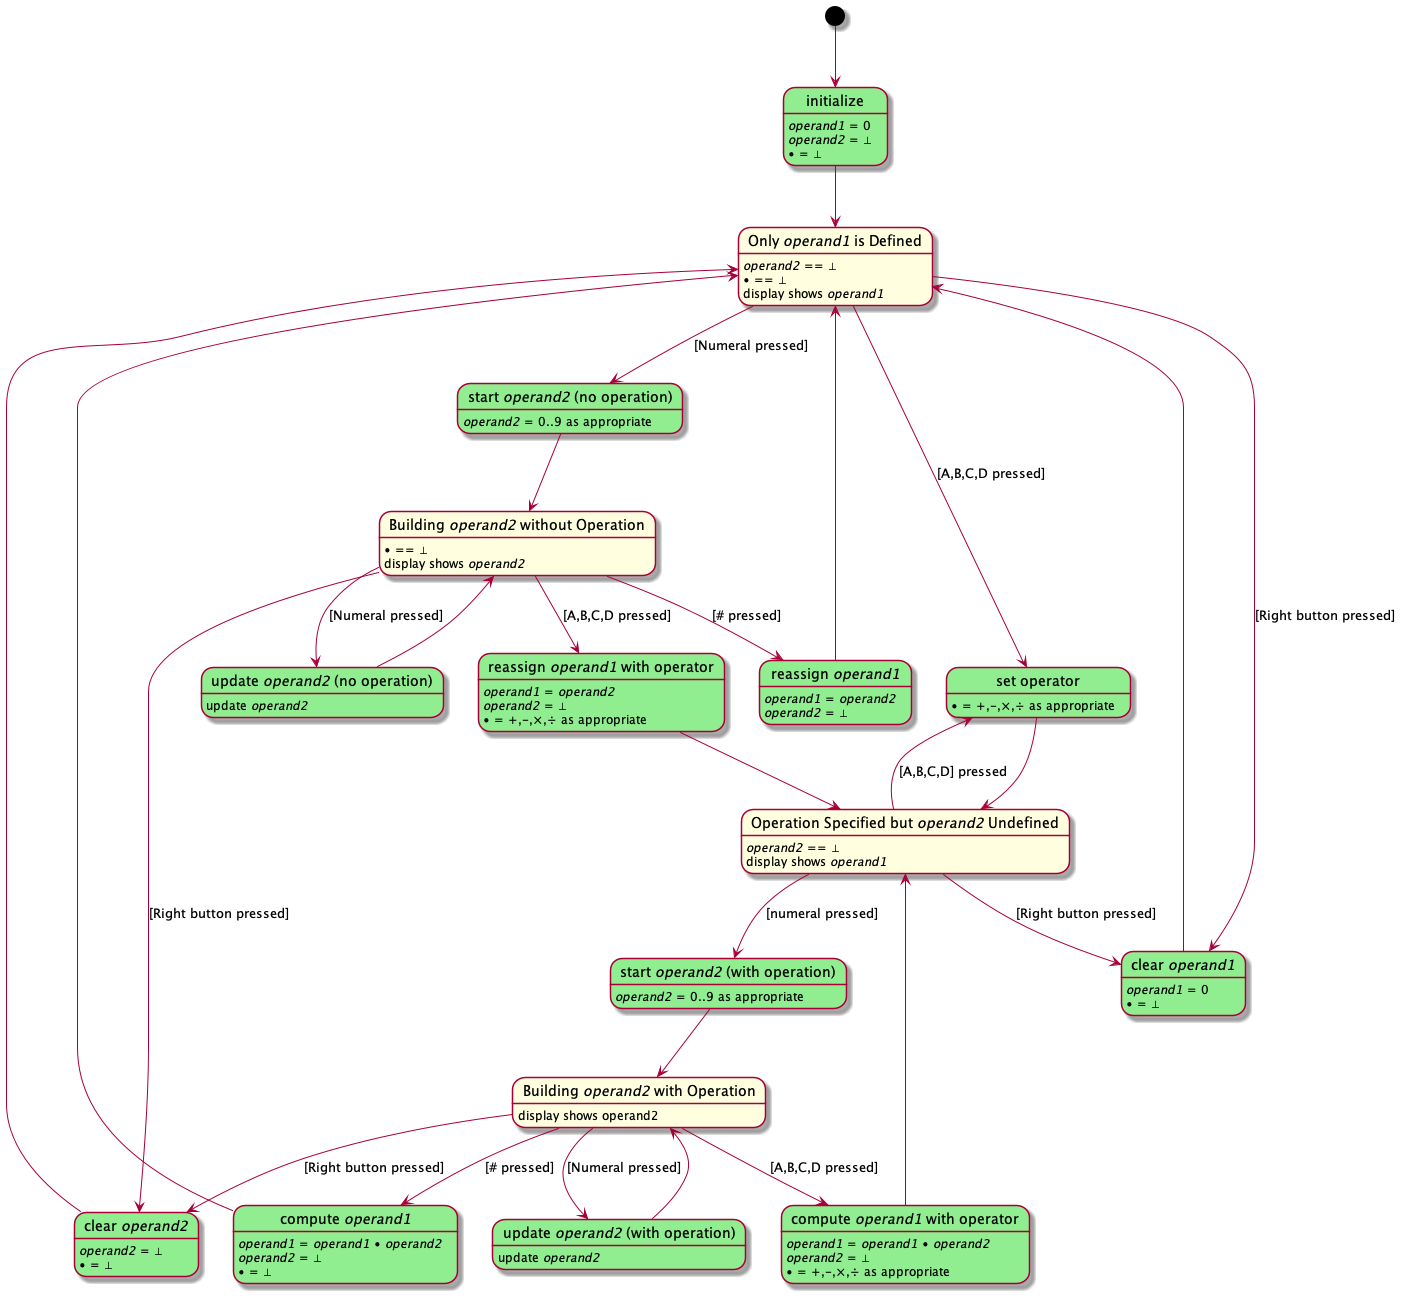
\includegraphics[width=18cm]{CalculatorStateDiagram}
    \caption{State diagram depicting ``normal'' behavior for integer calculator. Yellow states depict invariant conditions; green states depict updates to the problem-domain variables \textit{operand1}, \textit{operand2}, and $\bullet$ (operator). \tiny Diagram by Bohn \label{fig:StateDiagram}}
\end{figure}

% \subsection*{Fractional Calculator}
%
% If fractional-value behavior is implemented, then the calculator's
% specification is amended and extended:
%
% \begin{enumerate}[resume]
% \item Requirement~\ref{spec:NoDecimalPoint} is replaced with: \\
%     A decimal point shall be displayed as necessary:
%     \begin{enumerate}
%     \item The decimal point, when displayed, shall not occupy a full display
%         position in the \textbf{7-segment display module}; instead, it shall be
%         occupy the \texttt{DP} segment of the same display position as the
%         ones-place digit.
%     \item When \textit{operand1} is displayed, it shall always include a
%         decimal point.
%     \item When \textit{operand2} is displayed, the decimal point shall not be
%         displayed unless the \texttt{*} button has been pressed (see
%         requirement~\ref{spec:DecimalPointButton}).
%     \item If the value being displayed is an integer value and a decimal point
%         is required, then the decimal point shall be displayed after the
%         least-significant digit (for example: {\dviiseg 123.}). If the value
%         being displayed has a fractional portion, then the decimal point shall
%         be displayed between the ones-place and the tenths-place (for example,
%         $123\frac{1}{4}$ shall be displayed as {\dviiseg 123.25}).
%     \end{enumerate}
% \item The clarification sub-bullet for requirement~\ref{spec:IntegerCalculator}
%     is replaced with: \\
%     Division shall be conventional division; \textit{i.e.}, the fractional
%     portion of quotients, if any, shall be displayed in accordance with the
%     rounding rule of requirement~\ref{spec:Rounding}.
% \item Requirement~\ref{spec:LeadingZeroes} is amended: If the value to be
%     displayed is between -1.0 and 1.0, exclusive, then a {\dviiseg 0} shall be
%     displayed in the ones-place.
% \item Trailing 0s in the fractional portion of a value shall not be displayed.
%     For example, {\dviiseg 231.8} is correctly displayed, but {\dviiseg
%     231.80000} is not correctly displayed.
% \item \label{spec:DecimalPointButton} The \texttt{*} key can be thought of
%     as the decimal point key; that is, any keys pressed before pressing the
%     \texttt{*} key shall be part of the integer portion of the value being
%     built, and any keys pressed after pressing the \texttt{*} key shall be
%     part of the fractional portion of the value being built.
% \item \label{spec:Rounding} If the total number of digits required to display
%     the integer portion and the fractional portion of \textit{operand1}
%     (including the negative sign if needed) exceeds the number of digits in the
%     \textbf{7-segment display module}) then the value shall be rounded:
%     \begin{enumerate}
%     \item All display positions shall be used.
%     \item If the most-significant digit of the truncated portion is less than
%         5, then the value shall be rounded toward zero (\textit{i.e.}, the
%         least-significant displayed digit shall be unchanged). For example,
%         12345.6782 shall be displayed as {\dviiseg 12345.678} after rounding.
%     \item If the most-significant digit of the truncated portion is greater
%         than 5, or if that digit is 5 and there are more digits that follow,
%         then the value shall be rounded away from zero. For example, both
%         12345.6789 and 12345.67851 shall be displayed as {\dviiseg 12345.679}
%         after rounding.
%     \item If the most-significant digit of the truncated portion is 5 and there
%         are no digits that follow (``exactly halfway'') then the value shall be
%         rounded in whichever direction makes the least-significant displayed
%         digit even (0, 2, 4, 6, or 8). For example, both 12345.6775 and
%         12345.6785 shall be displayed as {\dviiseg 12345.678} after rounding.
%     \end{enumerate}
%     \begin{itemize}
%     \item If the value is too small to be displayed (the value is between
%         -0.0000005 and 0.00000005, inclusive, which round to 0) then {\dviiseg
%         0} shall be displayed. A negative value that rounds to 0 shall not
%         preserve its negative sign.
%     \item If the value is too great to be displayed after rounding (the
%         resulting integer portion requires more digits than are available) then
%         the value shall not be rounded; instead, {\dviiseg Error} shall be
%         displayed.
%     \end{itemize}
% \end{enumerate}

\section{Detecting Inputs} \label{sec:DetectingInputs}

Read Section~5 of the Cow Pi datasheet for an overview of handling interrupts for your \developmentboard.

To detect keypresses and buttonpresses, you will take advantage of having the NAND of the pushbuttons and the NAND of the keypad columns being input to Arduino pins D2 and D3.

Add code to \function{setup()} to register \function{handle_buttonpress()} as your buttonpress handler and \function{handle_keypress()} as your keypress handler.
Use the \function{attachInterrupt()} function described in Section~5.3 of the datasheet.

Initially, you don't have much for these functions to do -- you will add code to take appropriate action as you implement your system.
For now, place code in your \function{handle_buttonpress()} to illuminate the left LED when the left button is pressed and to illuminate the right LED when the right button is pressed.
You will later delete this code; this is simply to satisfy yourself that you are detecting the buttons being pressed and can determine which button has been pressed.
Similarly, add code to \function{handle_keypress()} to display the presed key on the display module.
You will alter delete this code; this is simply to satsify yourself that you are detecting keys being pressed and can determine which key has been pressed.

You will \textit{not} use interrupts to detect the switches changing position -- the specification has been written such that no action needs to be taken at the moment that a switch is toggled;
you only need to check the switch positions after something else has triggered some code.

\textbf{NOTE} Any global variables used by your interrupt handlers should be declared as \lstinline{volatile}.

Don't forget to reset the 7.5\mbox{-}second / 20\mbox{-}second countdown so that your code doesn't blank the display too soon.

Because we did not provide a hardware solution to switch bounce, you can expect
both the pin input to both rise and fall a few times when a button or key is
pressed and again when it is released -- but there is no guarantee that
bouncing will occur. For this reason we recommend:
    \begin{itemize}
    \item Use the \lstinline{CHANGE} mode, combined with software debouncing,
        and use a variable to keep track of whether a key or button has been
        pressed (toggle this variable whenever an interrupt occurs, and take
        action based on whether a key or button has been pressed or released).
    \item The software debouncing will look similar to what you used in
        PollingLab except that it only needs to be a few milliseconds instead
        of 500. Since we are not polling the buttons and keypad to detect
        presses, we do not need to worry about the button or key being held for
        several dozen milliseconds being interpretted as multiple presses.
        \begin{itemize}
        \item I very strongly advise against using \function{delay()} for
            software debouncing:
        \item As described in the PollingLab assignment sheet,
            \function{delay()} will leave your system unresponsive to anything
            except interrupts.
        \item Including \function{delay()} calls in an interrupt handler is
            particularly ill-advised since you may find yourself in a situation
            in which you need to disable interrupts in the interrupt handler
            and then re-enable interrupts before exiting the interrupt handler.
            (I do not expect this to happen in this assignment, but I've been
            wrong before.) The \function{delay()} function will never exit,
            blocking forever, if interrupts are disabled.
        \end{itemize}
    \end{itemize}
If you arrive at a different solution that works, you may use your solution.



\section{Implementing Timeout}\label{sec:TimerInterrupts}

Read Section~6 of the Cow Pi datasheet to familiarize yourself with timer interrupts on the \developmentboard.
Note that Sections~6.3--6.5 are generally duplicates of each other except for their tables and a warning at the start of Section~6.3;
for now you can read Sections~6.1, 6.2, 6.3, and 6.6.
Later, after you determine which timer you will use, you can re-visit Section~6.4 or 6.5 to consult its tables.

You must use timer interrupts from either Timer1 or Timer2 as part of your
implementation of the display timeout.
To implement the timeout, you will need to determine an appropriate timer period, from which you will determine the necessary comparison value and prescaler.
NOTE: there is no combination of interrupt period and comparison value to produce an interrupt period of 20~seconds, or even 7.5~seconds; you will need to use a shorter interrupt period with some other logic to determine when it is time to dim the displpay module.

Use the equation in the datasheet's Section~6.2 to iterate through possible comparison values and prescalers until you arrive at a prescaler that is available for one of the timers and a comparison value that fits in the available counter bits for that timer. When you have done so:
\begin{itemize}
    \item Uncomment the timer declaration on line~22 or 23, as appropriate, in the starter code
    \item Use the address offset listed in Section~6.4 or 6.5 to assign the approriate address to the \lstinline{timer} pointer in \function{setup()} on line 31
    \item Use the tables for your chosen timer to select the WGM bits for ``Clear on Timer Compare'' mode and the CS bits for your prescaler;
        use these bits to generate the bit vector that you will assign to \lstinline{timer->control} in \function{setup()} on line 32
    \item Subtract 1 from the comparison value and assign that to \lstinline{timer->compareA} in \function{setup()} on line 33
    \item Use the address offset listed in Section~6.6 to assign the appropriate address to the \lstinline{timer_interrupt_masks} pointer in \function{setup()} on line 34
    \item Create an ISR for the \texttt{TIMER\textit{n}\_COMPA\_vect} interrupt, where \texttt{n} is the timer number, using the \function{ISR()} macro as described in Section~5.2 of the datasheet;
        for now, write very simple code, such as turning an LED on or off, in the ISR --
        you will add useful code later
    \item Index the \lstinline{timer_interrupt_masks} array with the timer number and enable the \texttt{TIMER\textit{n}\_COMPA\_vect} interrupt, where \texttt{n} is the timer number, in \function{setup()} on line 35
\end{itemize}

Now you can add code to your ISR to implement your display-timeout logic.

\textbf{NOTE} Any global variables used by your ISR should be declared as \lstinline{volatile}.

\textbf{NOTE} If you ever need to ``reset'' a timer's count back to 0, you can
simply write 0 to the \lstinline{timer->counter} field.




\section{Turn-in and Grading}\addcontentsline{toc}{section}{Rubric}

When you have completed this assignment, upload \textit{CalculatorLab.ino} to
\filesubmission.

This assignment is worth 50 points. \\

Rubric:
\begin{description}
\rubricitem{2}{The source code is well-organized and is readable.}
\item[Pushbutton Interrupts]
\rubricitem{4}{Pushbutton presses are detected with an external interrupt.}
\rubricitem{2}{The pushbuttons' interrupt handler determines which button was pressed.}
% \rubricitem{4}{Pushbutton presses and releases are detected with an external
%     interrupt.}
% \rubricitem{2}{The pushbuttons' interrupt handler determines which button was
%     released.}
% \rubricitem{2}{The pushbuttons' interrupt handler determines whether the left
%     button has been double-clicked.}
\rubricitem{1}{Pushbutton interrupt handler is not excessively long.}
\item[Matrix Keypad Interrupts]
\rubricitem{4}{Matrix keypad presses are detected with an external interrupt.}
\rubricitem{2}{The keypad's interrupt handler determines which key was pressed.}
\rubricitem{1}{Keypad interrupt handler is not excessively long.}
\item[Timer Interrupts]
\rubricitem{2}{Timer interrupts for Timer1 or Timer2 are enabled and handled.}
\rubricitem{4}{The timer interrupts configured such that, when combined with
    other logic, the software is able to determine when exactly 7.5~seconds or
    exactly 20~seconds have passed.}
\rubricitem{1}{Timer ISR is not excessively long.}
\item[Timeout Logic]
% \rubricitem{2}{The system is able to determine when exactly 7.5~seconds have
%     passed since the left button was double-clicked.}
% \rubricitem{2}{The system is able to determine when exactly 20~seconds have
%     passed since the left button was double-clicked.}
\rubricitem{2}{The system is able to determine when exactly 7.5~seconds have
    passed since a button or key was pressed.}
\rubricitem{2}{The system is able to determine when exactly 20~seconds have
    passed since a button or key was pressed.}
\item[Normal Calculator Functionality]
\rubricitem{1}{Operand is built in accordance with
    requirements~\ref{spec:BuildingValue}, \ref{spec:Negative},
    \ref{spec:Positive}, and \ref{spec:LeadingZeroes}.}
% \rubricitem{1}{After eight digits (or a negative sign and seven digits),
%     subsequent numeral presses are ignored (except for resetting the
%     display-blanking countdown).}
\rubricitem{1}{After nine digits, subsequent numeral presses are ignored (except for resetting the display-blanking countdown).}
\rubricitem{2}{Addition performs correctly.}
\rubricitem{2}{Subtraction performs correctly.}
\rubricitem{2}{Multiplication performs correctly.}
\rubricitem{2}{Division performs correctly.}
\rubricitem{1}{The result of the previous arithmetic operation can be used as
    the first operand for the next arithmentic operation.}
\rubricitem{1}{The ``clear'' button clears the operand being built and any
    specified operation.}
\rubricitem{1}{If no operand is currently being built (the previous
    arithmetic's result is displayed) then the ``clear'' button clears the
    previous arithemtic's result and any specified operation.}
\rubricitem{1}{The result of the previous operation is displayed on the top row (if there was no previous operation, then \display{0}).}
\rubricitem{1}{The specified operation, if any, is displayed in the lower-left corner.}
\rubricitem{1}{The operand being built, if any, is displayed on the bottom row.}
\item[Other Calculator Functionality]
\rubricitem{1}{Too-great results cause \display{Error} to be displayed.}
% \rubricitem{2}{The display goes blank after exactly 7.5 seconds or exactly 20 seconds of inactivity, depending on the position of the left switch.}
% \rubricitem{2}{When the display is blank, pressing any button or key causes the display to resume\dots}
\rubricitem{2}{The display's backlight deluminates after exactly 7.5 seconds or exactly 20 seconds of inactivity, depending on the position of the left switch.}
\rubricitem{2}{When the display is dim, pressing any button or key causes the backlight to illuminate\dots}
\rubricitem{2}{\dots and has no other effect, allowing operation to resume where the user had left off before letting the display timeout.}
\item[Bonus]
% \bonusitem{5}{Fractional calculator is implemented.}
\bonusitem{2}{Get assignment checked-off by TA or professor during office hours before it is due. (Cannot get both bonuses.)}
\bonusitem{1}{Get assignment checked-off by TA at \textit{start} of your scheduled lab immediately after it is due. (Cannot get both bonuses.)}
\end{description}

\section*{Epilogue}

After using your calculator to compute how many specimens are still present in the lab, and establish that all specimens are accounted for after Newman's attempted theft.
As reports come in of facilities getting secured with Cow Pi-based locks and passages being monitored with Cow Pi-based motion sensors, Archie smiles and tells you that this was a job well done.
With all of the excitement neatly wrapped-up and arriving at a satisfactory conclusion, you look forward to a boring career in which there's absolutely no screaming and running for your life.

\textit{The End...?}

\newpage\appendix

\section{Lab Checkoff}

\textbf{NOTE: this checklist still needs to be updated to reflect changes for the new display module. An updated rubric will be released soon.}

You are not required to have your assignment checked-off by a TA or the
professor. If you do not do so, then we will perform a functional check
ourselves. In the interest of making grading go faster, we are offering a small
bonus %to get your assignment checked-off at the start of your scheduled lab
% time immediately after it is due. Because checking off all students during lab
% would take up most of the lab time, we are offering a slightly larger bonus
if you complete your assignment early and get it checked-off by a TA or the
professor during office hours.

\textit{Ideally, all team members are present for the check-off; however, only
one team member is necessary for the check-off.}

\begin{enumerate}
\item (\ \ \ ) Establish that the code you are demonstrating is the code you
    submitted to to \filesubmission.
    \begin{itemize}
    % \item If you are getting checked-off during lab time, show the TA that the
    %     file was submitted before it was due.
    \item Download the file into your PollingLab directory. If necessary,
        rename it to \textit{CalculatorLab.ino}.
    \end{itemize}
\item (\ \ \ ) Upload \textit{CalculatorLab.ino} to your \nano.
\item (\ \ \ ) If \textbf{Integer Calculator} then the display shows: \\
    {\dviiseg \phantom{8888888}0} \\
    % If \textbf{Fractional Calculator} then the display shows: \\
    %     {\dviiseg \phantom{8888888}0.} \\
    % \textit{Make a note of which calculator was implemented.}
\item (\ \ \ ) Place the left switch in the right position.
\item (\ \ \ ) Enter 123,456; the display shows: \\
    {\dviiseg \phantom{88}123456}
\item (\ \ \ ) \textbf{If you implemented display timeout:} Wait exactly five
    seconds. The display goes blank.
\item (\ \ \ ) \textbf{If you implemented display timeout:} Press 7. The display
    resumes, showing what it previously showed: \\
    {\dviiseg \phantom{88}123456}
\item (\ \ \ ) Press 7. The display shows: \\
    {\dviiseg \phantom{8}1234567}
\item (\ \ \ ) Press \texttt{A} (addition). The display still shows: \\
    {\dviiseg \phantom{8}1234567}
\item (\ \ \ ) Enter 890. The display shows: \\
    {\dviiseg \phantom{88888}890}
\item (\ \ \ ) Press \texttt{\#}. The display shows: \\
    {\dviiseg \phantom{8}1235457} \hspace{1cm} \textit{or} \hspace{1cm}
    {\dviiseg \phantom{8}1235457.}
\item (\ \ \ ) Press the right pushbutton (clear). The display shows: \\
    {\dviiseg \phantom{8888888}0} \hspace{1cm} \textit{or} \hspace{1cm}
    {\dviiseg \phantom{8888888}0.}
\item (\ \ \ ) Place the left switch in the left position.
\item (\ \ \ ) Enter -1,234,567, using the left pushbutton for the negative
    sign. The display shows: \\
    {\dviiseg -1235457}
\item (\ \ \ ) Press 8. The display still shows: \\
    {\dviiseg -1235457}
\item (\ \ \ ) Press \texttt{\#}. The display (still) shows: \\
    {\dviiseg -1235457} \hspace{1cm} \textit{or} \hspace{1cm}
    {\dviiseg -1234567.}
\item (\ \ \ ) Enter 231. The display shows: \\
    {\dviiseg \phantom{88888}231}
\item (\ \ \ ) Press \texttt{B} (subtraction) and enter 321. The display shows: \\
    {\dviiseg \phantom{88888}321}
\item (\ \ \ ) Press \texttt{\#}. The display shows: \\
    {\dviiseg \phantom{88888}-90} \hspace{1cm} \textit{or} \hspace{1cm}
    {\dviiseg \phantom{88888}-90.}
\item (\ \ \ ) Press the right pushbutton (clear). The display shows: \\
    {\dviiseg \phantom{8888888}0} \hspace{1cm} \textit{or} \hspace{1cm}
    {\dviiseg \phantom{8888888}0.}
\item (\ \ \ ) Press \texttt{C} (multiplication) and enter 12. The display
    shows:\\
    {\dviiseg \phantom{888888}12}
\item (\ \ \ ) Press \texttt{\#}. The display shows:\\
    {\dviiseg \phantom{8888888}0} \hspace{1cm} \textit{or} \hspace{1cm}
    {\dviiseg \phantom{8888888}0.}
\item (\ \ \ ) Enter 42. The display shows:\\
    {\dviiseg \phantom{888888}42}
\item (\ \ \ ) Press \texttt{D} (division) and enter 6. The display
    shows:\\
    {\dviiseg \phantom{8888888}6}
\item (\ \ \ ) Press \texttt{\#}. The display shows:\\
    {\dviiseg \phantom{8888888}7} \hspace{1cm} \textit{or} \hspace{1cm}
    {\dviiseg \phantom{8888888}7.}
\item (\ \ \ ) Press \texttt{C} (multiplication) and enter 73. The display
    shows:\\
    {\dviiseg \phantom{888888}73}
\item (\ \ \ ) Press \texttt{\#}. The display shows:\\
    {\dviiseg \phantom{88888}511} \hspace{1cm} \textit{or} \hspace{1cm}
    {\dviiseg \phantom{88888}511.}
\item (\ \ \ ) Press \texttt{C} (multiplication) and enter 200. The display
    shows:\\
    {\dviiseg \phantom{88888}200}
\item (\ \ \ ) Press the right pushbutton (clear). The display shows: \\
    {\dviiseg \phantom{88888}511} \hspace{1cm} \textit{or} \hspace{1cm}
    {\dviiseg \phantom{88888}511.}
\item (\ \ \ ) Press \texttt{C} (multiplication) and enter 200,000. The display
    shows:\\
    {\dviiseg \phantom{88}200000}
\item (\ \ \ ) Press \texttt{\#}. The display shows:\\
    {\dviiseg \phantom{88}Error}
\item (\ \ \ ) \textbf{If you implemented display timeout:}
    \begin{description}
    \item [[ ]] Show the code in which you configured Timer1 or Timer2
    \item [[ ]] Explain the calculation that you used to arrive at your
        comparison value
        \[comparison\_value = 16,000,000 \times interrupt\_period \div prescaler\]
    \item [[ ]] Show and explain the Timer ISR
    \item [[ ]] Show and explain any other code used to implement the display
        timeou
    \item [[ ]] Show and explain the Timer ISR.
    \item [] \textit{If it is not clear to the TA how the display-timeout code
        works, then the TA will:}
    \item [[ ]] Prepare a stopwatch or another timepiece with a ``seconds''
        display (or a ``seconds'' hand)
    \item [[ ]] If necessary, re-activate the display by pressing a button or
        key
    \item [[ ]] Press a button or key on the system at the exact same time as
        starting the stopwatch (or at the exact moment that the ``seconds''
        display/hand hits \textit{00})
    \item [[ ]] Note whether the display clears at exactly 30 seconds and not
        at 30.7 seconds, 29.7 seconds, nor any other that would suggest that
        \function{millis()} is used in the display timeout implementation
    \end{description}
\item (\ \ \ ) Show and explain the code used to register the external
    interrupt handlers
\item (\ \ \ ) Show and explain the pushbutton interrupt handler
\item (\ \ \ ) Show and explain the keypad interrupt handler
\item (\ \ \ ) Show the start of \textit{CalculatorLab.ino} to show the TA that the only \lstinline{#include}d header files are \textit{cowpi.h} and possibly the header file(s) from one or more of the Arduino standard libraries.
\end{enumerate}

% If you implemented \textbf{Integer Calculator}, then this concludes the
% demonstration of your system's functionality. These steps are written to detect
% constraint violations during the check-off; however, the TAs will later examine
% your code for violations of the assignment's constraints.
% \begin{itemize}
% \item If we find that your display timeout uses Timer0 or uses code that uses
% Timer0 (such as \function{millis()}, \function{micros()}, or
% \function{delay()}) then you will lose any points that you received for the
% display timeout functionality.
% \item If we find that your code polls the pushbuttons to detect button presses
% then you will lose any points that you received for implementing the pushbutton
% handler.
% \item If we find that your code polls the matrix keypad to detect key presses
% then you will lose any points that you received for implementing the keypad
% handler.
% \item If we find that you used a third-party library then you will lose any
% points that you received for functionality that made use of that library.
% \end{itemize}

% If you implemented \textbf{Fractional Calculator}:
%
% \begin{enumerate}[resume]
% \item (\ \ \ ) Enter 3.5, using the \texttt{*} key for the decimal point. The
%     display shows: \\
%     {\dviiseg \phantom{888888}3.5}
% \item (\ \ \ ) Press \texttt{B} (subtraction) and enter 2.8. The display shows: \\
%     {\dviiseg \phantom{888888}2.8}
% \item (\ \ \ ) Press \texttt{\#}. The display shows: \\
%     {\dviiseg \phantom{888888}0.7}
% \item (\ \ \ ) Press \texttt{A} (addition) and enter 10.32. The display shows: \\
%     {\dviiseg \phantom{8888}10.32}
% \item (\ \ \ ) Press \texttt{\#}. The display shows: \\
%     {\dviiseg \phantom{8888}11.02}
% \item (\ \ \ ) Press \texttt{C} (multiplication) and enter 23.9. The display shows: \\
%     {\dviiseg \phantom{88888}23.9}
% \item (\ \ \ ) Press \texttt{\#}. The display shows: \\
%     {\dviiseg \phantom{88}263.378}
% \item (\ \ \ ) Press \texttt{A} (addition) and enter 100,000. The display
%     shows: \\
%     {\dviiseg \phantom{88}100000}
% \item (\ \ \ ) Press \texttt{\#}. The display shows: \\
%     {\dviiseg 100263.38}
% \item (\ \ \ ) Enter 22.9. The display shows: \\
%     {\dviiseg \phantom{88888}22.9}
% \item (\ \ \ ) Press \texttt{D} (division) and enter 5.4. The display shows: \\
%     {\dviiseg \phantom{888888}5.4}
% \item (\ \ \ ) Press \texttt{\#}. The display shows: \\
%     {\dviiseg 4.2407407}
% \item (\ \ \ ) Enter 25.5. The display shows: \\
%     {\dviiseg \phantom{88888}25.5}
% \item (\ \ \ ) Press \texttt{D} (division) and enter 4. The display shows: \\
%     {\dviiseg \phantom{8888888}4}
% \item (\ \ \ ) Press \texttt{\#}. The display shows: \\
%     {\dviiseg \phantom{8888}6.375}
% \item (\ \ \ ) Press \texttt{D} (division) and enter 100. The display shows: \\
%     {\dviiseg \phantom{88888}100}
% \item (\ \ \ ) Press \texttt{\#}. The display shows: \\
%     {\dviiseg \phantom{88}0.06375}
% \item (\ \ \ ) Press \texttt{D} (division) and enter 10,000,000. The display
%     shows: \\
%     {\dviiseg 10000000}
% \item (\ \ \ ) Press \texttt{\#}. The display shows: \\
%     {\dviiseg \phantom{8888888}0.}
% \end{enumerate}

This concludes the demonstration of your system's functionality. These steps
are written to detect constraint violations during the check-off; however, the
TAs will later examine your code for violations of the assignment's constraints
and deduct any unearned points accordingly.

\end{document}
